\achapter{37}{Linear Transformations} \label{chap:linear_transformation}

\vspace*{-17 pt}
\framebox{
\parbox{\dimexpr\linewidth-3\fboxsep-3\fboxrule}
{\begin{fqs}
\item What is a linear transformation?
\item What is the kernel of a linear transformation? What algebraic structure does a kernel of a linear transformation have? 
\item What is a one-to-one linear transformation? How does its kernel tell us if a linear transformation is one-to-one?
\item What is the range of a linear transformation? What algebraic property does the range of a linear transformation possess? 
\item What is an onto linear transformation? What relationship is there between the codomain and range if a linear transformation is onto?
\item What is an isomorphism of vector spaces?
\end{fqs}}}% \hspace*{3 pt}}

\vspace*{13 pt}

\csection{Application: Fractals}    
\label{sec:appl_fractals}   

Sierpinski triangles and Koch's curves have become common phrases in many mathematics departments across the country. These objects are examples of what are called \emph{fractals}, beautiful geometric constructions that exhibit self-similarity.  Fractals are applied in a variety of ways: they help make smaller antennas (e.g., for cell phones) and are used in fiberoptic cables, among other things. In addition, fractals can be used to model realistic objects, such as the Black Spleenwort fern depicted as a fractal image in Figure \ref{F:Fern}. As we will see later in this section, one way to construct a fractal is with an \emph{Iterated Function System} (IFS). 
\begin{figure}[h]
\begin{center}
\resizebox{!}{1.5in}{\includegraphics{Fern}}
\caption{An approximation of the Black Spleenwort fern.}
\label{F:Fern}
\end{center}
\end{figure}

\csection{Introduction}
\label{sec:lin_trans_intro}

We have encountered functions throughout our study of mathematics -- we explore graphs of functions in algebra and differentiate and integrate functions in calculus. In linear algebra we have investigated special types of functions, e.g., matrix and coordinate transformations, that preserve the vector space structure. Any function that has the same properties as matrix and coordinate transformations is a \emph{linear transformation}. Linear transformations are important in linear algebra in that we can study similarities and connections between vector spaces by examining transformations between them. Linear transformations model or approximately model certain real-life processes (like discrete dynamical systems, geometrical transformations, Google PageRank, etc.). Also, we can determine the behavior of an entire linear transformation  by knowing how it acts on just a basis.

\begin{definition} A \textbf{linear transformation}\index{linear transformation} from a vector space $V$ to a vector space $W$ is a function $T: V \to W$ such that
\begin{enumerate}
\item $T(\vu + \vv) = T(\vu) + T(\vv)$ and
\item $T(c\vv) = cT(\vv)$
\end{enumerate}
for all $\vu, \vv$ in $V$ and all scalars $c$.
\end{definition}

These transformations are called \emph{linear} because they respect linear combinations. We can combine both parts of this definition into one statement and say that a mapping $T$ from a vector space $V$ to a vector space $W$ is a linear transformation if
\[T(a\vu + b \vv) = aT(\vu) + bT(\vv)\]
for all vectors $\vu, \vv$ in $V$ and all scalars $a$ and $b$. We can extend this property of a linear transformation (by mathematical induction) to any finite linear combination of vectors. That is, if $\vv_1$, $\vv_2$, $\ldots$, $\vv_k$ are any vectors in the domain of a linear transformation $T$ and $c_1$, $c_2$, $\ldots$, $c_k$ are any scalars, then
\[T(c_1 \vv_1 + c_2 \vv_2 + \cdots + c_k \vv_k) = c_1 T(\vv_1) + c_2 T(\vv_2) + \cdots + c_k T(\vv_k).\]
This is the property that $T$ respects linear combinations.

\begin{pa} \label{pa:8_a} ~
	\be
	\item Consider the transformation $T: \R^3 \to \R^2$ defined by 
	\[T\left( \left[ \begin{array}{cc} x\\y\\z \end{array} \right] \right) = \left[ \begin{array}{c} x+y\\z+3 \end{array} \right]\]
Check that $T$ is not linear by finding two vectors $\vu, \vv$ which violate the additive property of linear transformations.
	
		\item  Consider the transformation $T : \pol_2 \to \pol_3$ defined by
	\[T(a_0+a_1t+a_2t^2) = (a_0+a_1) + a_2t + a_1t^3\]
Check that $T$ is a linear transformation.

	\item Let $\D$ be the set of all differentiable functions from $\R$ to $\R$. Since $\frac{d}{dx}(0) = 0$, $(f+g)'(x) = f'(x)+g'(x)$ and $(cf)'(x) = cf'(x)$ for any differentiable functions $f$ and $g$ and any scalar $c$, it follows that $\D$ is a subspace of $\F$, the vector space of all functions from $\R$ to $\R$. Let $T: \D \to \F$ be defined by $T(f) = f'$. Check that $T$ is a linear transformation.
		
	\item Every matrix transformation is a linear transformation, so we might expect that general linear transformations share some of the properties of matrix transformations. Let $T$ be a linear transformation from a vector space $V$ to a vector space $W$. Use the linearity properties to show that $T(\vzero_V) = \vzero_W$,  where $\vzero_V$ is the additive identity in $V$ and $\vzero_W$ is the additive identity in $W$. (Hint: $0_V + 0_V = 0_V$.)


\ee

\end{pa}

\csection{Onto and One-to-One Transformations}
\label{sec:onto_oneone}

Recall that in Section \ref{sec:matrix_transformations} we expressed existence and uniqueness questions for matrix equations in terms of one-to-one and onto properties of matrix transformations. The question about the existence of a solution to the matrix equation $A \vx = \vb$ for any vector $\vb$, where $A$ is an $m \times n$ matrix, is also a question about the existence of a vector $\vx$ so that $T(\vx) = \vb$, where $T(\vx) = A \vx$. If, for each $\vb$ in $\R^m$ there is at least one $\vx$ with $T(\vx) = \vb$, then $T$ is an onto transformation. We can make a similar definition for any linear transformation. 

\begin{definition} A linear transformation $T$ from a vector space $V$ to a vector space $W$ is \textbf{onto}\index{linear transformation!onto} if each $\vb$ in $W$ is the image of at least one $\vx$ in $V$.
\end{definition}

Similarly, the uniqueness of a solution to $A \vx = \vb$ for any $\vb$ in $\Col A$ is the same as saying that for any $\vb$ in $\R^m$, there is at most one $\vx$ in $\R^n$ such that $T(\vx) = \vb$. A matrix transformation with this property is one-to-one, and we can make a similar definition for any linear transformation. 

\begin{definition} A linear transformation $T$ from a vector space $V$ to a vector space $W$ is \textbf{one-to-one}\index{linear transformation!onto} if each $\vb$ in $W$ is the image of at most one $\vx$ in $V$.
\end{definition}

With matrix transformations we saw that there are easy pivot criteria for determining whether a matrix transformation is one-to-one (a pivot in each column) or onto (a pivot in each row). If a linear transformation can be represented as a matrix transformation, then we can use these ideas. However, not every general linear transformation can be easily viewed as a matrix transformation, and in those cases we might have to resort to applying the definitions directly.

\begin{activity}
For each of the following transformations, determine if $T$ is one-to-one and/or onto.
	\ba
	\item $T: \pol_2 \to \pol_1$ defined by $T(a_0+a_1t+a_2t^2) = a_0+(a_1+a_2)t$.
	\item $T: \D \to \F$ defined by $T(f) = f'$.
	\ea
\end{activity}



\csection{The Kernel and Range of Linear Transformation}
\label{sec:kernel_range}

As we saw in Preview Activity \ref{pa:8_a}, any linear transformation sends the additive identity to the additive identity. If $T$ is a matrix transformation defined by $T(\vx) = A \vx$ for some $m \times n$ matrix $A$, then we have seen that the set of vectors that $T$ maps to the zero vector is $\Nul A = \{\vx : A \vx = \vzero\}$, which is also $\Ker(T) = \{\vx : T(\vx) = \vzero\}$. We can extend this idea of the kernel of a matrix transformation to any linear transformation $T$. 

\begin{definition} Let $T : V \to W$ be a linear transformation from the vector space $V$ to the vector space $W$. The \textbf{kernel}\index{linear transformation!kernel} of $T$ is the set
\[\Ker(T) = \{\vx \in V : T(\vx) = \vzero_W\},\]
where $\vzero_W$ is the additive identity in $W$.
\end{definition}

Just as the null space of an $m \times n$ matrix $A$ is a subspace of $\R^n$, the kernel of a linear transformation from a vector space $V$ to a vector space $W$ is a subspace of $V$. The proof is left to the exercises.  

\begin{theorem} \label{thm:8_a_ker} Let $T : V \to W$ be a linear transformation from a vector space $V$ to vector space $W$. Then $\Ker(T)$ is a subspace of $V$.
\end{theorem}


The kernel of a linear transformation provides a convenient way to determine if the linear transformation is one-to-one. If $T$ is one-to-one, then the only solution to $T(\vx) = \vzero_W$ is $\vzero_V$ and $\Ker(T)$ contains only the zero vector. If $T$ is not one-to-one (and the domain of $T$ is not just $\{\vzero\}$), then the number of solutions to $T(\vx) = \vzero_W$ is infinite and $\Ker(T)$ contains more than just the zero vector. We formalize this idea in the next theorem. (Compare to Theorem \ref{thm:3_b_one_to_one_kernel}.) The formal proof is left for the exercises. 

\begin{theorem} \label{thm:8_a_one_to_one_kernel} A linear transformation $T$ from a vector space $V$ to a vector space $W$ is one-to-one if and only if $\Ker(T) = \{\vzero_V\}$, where $\vzero_V$ is the additive identity in $V$.
\end{theorem}


\begin{activity}  \label{act:8_a_Lin_trans_1} ~
\ba
\item Let $T: \pol_1 \to \pol_2$ be defined by $T(a_0+a_1t) = a_1t^2$. Find $\Ker(T)$. Is $T$ one-to-one? Explain.
\item Let $T: \D \to \F$ be defined by $T(f) = f'$. Find $\Ker(T)$.
\ea
\end{activity}

Recall that the matrix-vector product $A \vx$ is a linear combination of the columns of $A$ and the set of all vectors of the form $A \vx$ is the column space of $A$. For the matrix transformation $T$ defined by $T(\vx) = A\vx$, the set of all vectors of the form $A \vx$ is also the range of the transformation $T$. We can extend this idea to arbitrary linear transformations to define the \emph{range} of a transformation. 

\begin{definition} Let $T : V \to W$ be a linear transformation from the vector space $V$ to the vector space $W$. The \textbf{range}\index{range of a linear transformation} of $T$ is the set
\[\Range(T) = \{T(\vx) : \vx \text{ is in } V\}.\]
\end{definition}

We also call the range of a transformation $T$ the \emph{image}\index{image of a linear transformation}  of the transformation and use the notation $\Image(T)$. 

If $T(\vx) = A\vx$ for some $m \times n$ matrix $A$, we know that $\Col A$, the span of the columns of $A$, is a subspace of $\R^m$. Consequently, the range of $T$, which is also the column space of $A$, is a subspace of $\R^m$. In general, the range of a linear transformation $T$ from $V$ to $W$ is a subspace of $W$. The fact that the range of a transformation is a subspace of the codomain is a consequence of the more general result in the following theorem.

\begin{theorem} Let $T : V \to W$ be a linear transformation from a vector space $V$ to vector space $W$, and let $U$ be a subspace of $V$. Then the set 
\[T(U) = \{T(\vu) : \vu \in U\}\]
is a subspace of $W$.
\end{theorem}

\begin{proof} Let $T : V \to W$ be a linear transformation from a vector space $V$ to vector space $W$, and let $U$ be a subspace of $V$. Let $\vzero_V$ and $\vzero_W$ be the additive identities in $V$ and $W$, respectively. We have already shown that $T(\vzero_V) = \vzero_W$, so $\vzero_W$ is in $T(U)$. To show that $T(U)$ is a subspace of $W$ we must also demonstrate that $\vw+\vz$ is in $T(U)$ whenever $\vw$ and $\vz$ are in $T(U)$ and that $a\vw$ is in $T(U)$ whenever $a$ is a scalar and $\vw$ is in $T(U)$. Let $\vw$ and $\vz$ be in $T(U)$. Then $T(\vx) = \vw$ and $T(\vy) = \vz$ for some vectors $\vx$ and $\vy$ in $U$. Since $U$ is a subspace of $V$, we know that $\vx+\vy$ is in $U$. The fact that $T$ is a linear transformation means that
\[T(\vx + \vy) = T(\vx) + T(\vy) = \vw + \vz.\]
So $\vw+\vz$ is in $T(U)$.

Finally, let $a$ be a scalar. Since $U$ is a subspace of $V$, we know that $a \vx$ is in $U$. The linearity of $T$ gives us
\[T(a\vx) = aT(\vx) = a\vw,\]
so $a \vw$ is in $T(U)$.  We conclude that $T(U)$ is a subspace of $W$.
\end{proof}

Letting $U = V$ shows that $\Range(T)$ is a subspace of $W$. 

The subspace $\Range(T)$ provides us with a convenient criterion for the transformation $T$ being onto. The transformation $T$ is onto if for each $\vb$ in $W$, there is at least one $\vx$ for which $T(\vx)=\vb$. This means that every $\vb$ in $W$ belongs to $\Range(T)$ for $T$ to be onto. 

\begin{theorem} \label{thm:8_a_onto_range} A linear transformation $T$ from a vector space $V$ to a vector space $W$ is onto if and only if $\Range(T) = W$.
\end{theorem}

\begin{activity}  Let $T: \pol_1 \to \pol_2$ be defined by $T(a_0+a_1t) = a_1t^2$ as in Activity \ref{act:8_a_Lin_trans_1} . Describe the vectors in $\Range(T)$. Is $T$ onto? Explain.

\end{activity}

\csection{Isomorphisms}
\label{sec:isomorph}

If $V$ is a vector space with a basis $\CB = \{\vv_1, \vv_2, \ldots, \vv_n\}$, we have seen that the coordinate transformation $T : V \to \R^n$ defined by $T(\vx) = [\vx]_{\CB}$ is a linear transformation that is both one-to-one and onto. This allows us to uniquely identify any vector in $V$ with a vector in $\R^n$ so that the vector space structure is preserved. In other words, the vector space $V$ is for all intents and purposes the same as the vector space $\R^n$, except for the way we represent the vectors. This is a very powerful idea in that it shows that any vector space of dimension $n$ is essentially the same as $\R^n$. 
 When this happens we say that the vectors spaces are \emph{isomorphic} and call the coordinate transformation an \emph{isomorphism}.

\begin{definition}  An \textbf{isomorphism}\index{isomorphism} from a vector space $V$ to a vector space $W$ is a linear transformation $T : V \to W$ that is one-to-one and onto. 
\end{definition}

We this terminology, we summarize the discussion in the following theorem.

\begin{theorem} If $V$ is a vector space of dimension $n$, then any coordinate transformation from $V$ to $\R^n$ is an isomorphism.
\end{theorem}

It is left for the exercises to show that if $T: V \to W$ is an isomorphism, then $T^{-1}: W \to V$ is also an isomorphism. So if there is an isomorphism from a vector space $V$ to a vector space $W$, then there is an isomorphism from $W$ to $V$. As a result, we say that $V$ and $W$ are \emph{isomorphic} vector spaces\index{vector spaces!isomorphic}. It is also true that any vector space is isomorphic to itself, and that if $V$ is isomorphic to $W$ and $W$ is isomorphic to $U$, then $V$ and $U$ are also isomorphic. The proof of this result is left to the exercises. From this last property we can conclude that any two vector spaces of dimension $n$ are isomorphic vector spaces. This validates statement we made earlier that the vector space $\pol_n$ is for all intents and purposes the same as $\R^{n+1}$, since the two spaces are isomorphic. So to understand all finite dimensional vector spaces, it is enough to understand $\R^n$. The next activity provides a little practice with isomorphisms. 

\begin{activity} Assume that each of the following maps is a linear transformation. Which, if any, is an isomorphism? Justify your reasoning.
	\ba
	\item $T: \pol_1 \to \R^2$ defined by $T(a_0+a_1t) = \left[ \begin{array}{c} a_1\\a_1+a_0 \end{array} \right]$
	\item $T: \M_{2 \times 2} \to \pol_3$ defined by $T\left(\left[ \begin{array}{cc} a&b\\ c&d \end{array} \right] \right) = a+bt+ct^2+dt^3$. 
	\item $T: \R^2 \to \pol_2$ defined by $T\left(\left[ \begin{array}{c} a\\ b \end{array} \right] \right) = a+bt+at^2$.
	\ea
	
\end{activity}



\csection{Examples} 
\label{sec:lin_trans_exam}

\ExampleIntro

\begin{example} Let $T : \pol_2 \to \pol_3$ be defined by $T(p(t)) = tp(t)+p(0)$.
\ba
\item Show that $T$ is a linear transformation.

\item Is $T$ one-to-one? Justify your answer. 

\item 
	\begin{enumerate}[i.]
	\item Find three different polynomials in $\Range(T)$. 
	
	\item Find, if possible, a polynomial that is not in $\Range(T)$. 
	
	\item Describe $\Range(T)$. What is $\dim(\Range(T))$? Is $T$ an onto transformation? Explain. 
	\end{enumerate}

\ea

\ExampleSolution

\ba
\item To show that $T$ is a linear transformation we must show that $T(p(t)+q(t)) = T(p(t)) + T(q(t))$ and $T(cp(t)) = cT(p(t))$ for every $p(t)$, $q(t)$ in $\pol_2$ and any scalar $c$. Let $p(t)$ and $q(t)$ be in $\pol_2$. Then 
\begin{align*}
T(p(t)+q(t)) &= t(p(t)+q(t)) + (p(0)+q(0)) \\
	&= \left(tp(t) + p(0)\right) + \left( tq(t) + q(0) \right) \\
	&= T(p(t)) + T(q(t))
\end{align*}
and 
\[T(cp(t)) = tcp(t) + cp(0) = c\left(tp(t)+p(0)\right) = cT(p(t)).\]
Therefore, $T$ is a linear transformation.

\item To determine if $T$ is one-to-one, we find $\Ker(T)$. Suppose $p(t) = a_0+a_1t+a_2t^2  \in \Ker(T)$. Then 
\[0 = T(p(t)) = tp(t) + p(0) =  a_0t+a_1t^2 +a_2t^3 + a_0. \]
Equating coefficients on like powers of $t$ shows that $a_0 = a_1 = a_2 = 0$. Thus, $p(t) = 0$ and $\Ker(T) = \{0\}$. Thus, $T$ is one-to-one.

\item 
	\begin{enumerate}[i.]
	\item We can find three polynomials in $\Range(T)$ by applying $T$ to three different polynomials in $\pol_2$. So three polynomials in $\Range(T)$ are
	\begin{align*}
	T(1) &= t+1  \\
	T(t) &= t^2 \\
	T\left(t^2\right) &= t^3.
	\end{align*}
	
	\item A polynomial $q(t) = b_0+b_1t+b_2t^2+b_3t^3$ is in $\Range(T)$ if $q(t) = T(p(t))$ for some polynomial $p(t) = a_0+a_1t+a_2t^2$ in $\pol_2$. This would require that 
	\[b_0+b_1t+b_2t^2+b_3t^3 = a_0t+a_1t^2+a_2t^3+a_0.\]
	But this would mean that $b_0 = a_0 = b_1$. So the polynomial $1+2t+t^2+t^3$ is not in $\Range(T)$. 	
		
	\item Let $q(t)$ be in $\Range(T)$. Then $q(t) = T(p(t))$ for some polynomial $p(t) = a_0+a_1t+a_2t^2 \in \pol_2$. Thus,
\begin{align*}
q(t) &= T(p(t)) \\
	&= tp(t) + p(0) \\
	&= a_0t+a_1t^2+a_2t^3 + a_0 \\
	&= a_0(t+1) + a_1t^2 +a_2t^3.
\end{align*}
Therefore, $\Range(T) = \Span\{t+1, t^2, t^3\}$. Since the reduced row echelon form of $\left[ \begin{array}{ccc} 1&0&0\\1&0&0\\0&1&0\\0&0&1 \end{array} \right]$ is $\left[ \begin{array}{ccc} 1&0&0\\0&1&0\\0&0&1\\0&0&0 \end{array} \right]$, we conclude that the set $\{t+1, t^2, t^3\}$ is linearly independent. Thus, $\dim(\Range(T)) = 3$. Since $\Range(T)$ is a three-dimensional subspace of the four-dimensional space $\pol_3$, it follows that $T$ is not onto. 

	\end{enumerate}
\ea

\end{example}


\begin{example} Let $T: \M_{2 \times 2} \to \pol_3$ be defined by 
\[T\left( \left[ \begin{array}{cc} a&b\\c&d \end{array} \right] \right) = a+bt+ct^2+dt^3.\]
Show that $T$ is an isomorphism from $\M_{2 \times 2}$ to $\pol_3$.

\ExampleSolution

We need to show that $T$ is a linear transformation, and that $T$ is both one-to-one and onto. We start by demonstrating that $T$ is a linear transformation. Let $A = [a_{ij}]$ and $B = [b_{ij}]$ be in $\M_{2 \times 2}$. Then
\begin{align*}
T(A+B) &= T\left([a_{ij}+b_{ij}]\right) \\
	&= \left(a_{11}+b_{11}\right) + \left(a_{12}+b_{12}\right)t + \left(a_{21}+b_{21}\right)t^2 + \left(a_{22}+b_{22}\right)t^3 \\
	&= \left(a_{11}+a_{12}t+a_{21}t^2+a_{22}t^3\right)  +  \left(b_{11}+b_{12}t+b_{21}t^2+b_{22}t^3\right) \\
	&= T(A) + T(B).
\end{align*}
Now let $c$ be a scalar. Then
\begin{align*}
T(cA) &= T\left([ca_{ij}]\right) \\
	&= \left(ca_{11}\right)+\left(ca_{12}\right)t+\left(ca_{21}\right)t^2+\left(ca_{22}\right)t^3 \\
	&= c\left(a_{11}+a_{12}t+a_{21}t^2+a_{22}t^3\right) \\
	&= cT(A).
\end{align*}
Therefore, $T$ is a linear transformation.

Next we determine $\Ker(T)$. Suppose $A \in \Ker(T)$. Then 
\[0 = T(A) = a_{11}+a_{12}t+a_{21}t^2+a_{22}t^3.\]
Equating coefficients of like powers of $T$ shows that $a_{ij} = 0$ for each $i$ and $j$. Thus, $A = 0$ and $\Ker(T) = \{0\}$. It follows that $T$ is one-to-one.

Finally, we show that $\Range(T) = \pol_3$. If $q(t) = a+bt+ct^2+dt^3 \in \pol_3$, then $T\left( \left[ \begin{array}{cc} a&b\\c&d \end{array} \right] \right) = q(t)$. So every polynomial in $\pol_3$ is the image of some matrix in $\M_{2 \times 2}$. It follows that $T$ is onto and also that $T$ is an isomorphism. 
  
\end{example}



\csection{Summary}
\label{sec:lin_trans_summ}
Let $T$ be a linear transformation from a vector space $V$ to a vector space $W$. 
\begin{itemize}
\item A function $T$  from a vector space $V$ to a vector space $W$ is a linear transformation if 
	\be
	\item $T(\vu + \vv) = T(\vu) + T(\vv)$ for all $\vu$ and $\vv$ in $V$ and
	\item $T(c\vu) = cT(\vu)$ for all $\vu$ in $V$ and all scalars $c$.
	\ee
\item Let $T$ be a linear transformation from a vector space $V$ to a vector space $W$. The kernel of $T$ is the set
\[\Ker(T) = \{\vx \in V : T(\vx) = \vzero\}.\]
The kernel of $T$ is a subspace of $V$.
\item Let $T$ be a linear transformation from a vector space $V$ to a vector space $W$. The transformation $T$ is one-to-one if every vector in $W$ is the image under $T$ of at most one vector in $V$. A linear transformation $T$ is one-to-one if and only if $\Ker(T) = \{\vzero\}$.
\item Let $T$ be a linear transformation from a vector space $V$ to a vector space $W$. The range of $T$ is the set 
\[\Range(T) = \{T(\vv) : \vv \in V\}.\]
The range of $T$ is a subspace of $W$.
\item Let $T$ be a linear transformation from a vector space $V$ to a vector space $W$. The linear transformation $T$ is onto if every vector in $W$ is the image under $T$ of at least one vector in $V$. The transformation $T$ is onto if and only if $\Range(T) = W$.
\item An isomorphism from a vector space $V$ to a vector space $W$ is a linear transformation $T : V \to W$ that is one-to-one and onto. 
\end{itemize}

\csection{Exercises}
\label{sec:lin_trans_exer}
\be

\item We have seen that $C[a,b]$, the set of all continuous functions on the interval $[a,b]$ is a vector space. Let $T : C[a,b] \to \R$ be defined by $T(f) = \int_a^b f(x) \, dx$. 
Show that $T$ is a linear transformation. 

\item \label{ex:8_a_reflexive_isomorphism}  If $V$ is a vector space, prove that the identity map $I:V \to V$ defined by $I(\vx) = \vx$ for all $\vx \in V$ is an isomorphism.


\item \label{ex:8_a_inverse_isomorphism} Let $V$ and $W$ be vector spaces and let $T : V \to W$ be an isomorphism.  Since $T$ is a bijection, $T$ has an inverse function. (Recall that two functions $f$ and $g$ are inverses if $(f \circ g)(x) = x$ for all $x$ in the domain of $g$ and $(g \circ f)(x) = x$ for all $x$ in the domain of $f$.)
\ba
\item Let $T: \pol_1 \to \R^2$ be defined by $T(a_0+a_1t) = \left[ \begin{array}{c} a_0\\a_0+a_1 \end{array} \right]$. Assume that $T$ is an isomorphism. Show that $S: \R^2 \to \pol_1$ defined by $S([a \ b]^{\tr}) = a + (b-a)t$ is the inverse of $T$. 

\item Let $T: \M_{2 \times 2} \to \pol_3$ be defined by $T\left(\left[ \begin{array}{cc} a&b\\ c&d \end{array} \right] \right) = a+bt+ct^2+dt^3$. Assume that $T$ is an isomorphism. Find the inverse of $T$. Make sure to verify that your conjectured function really is the inverse of $T$. 
	
\item Now assume that $T$ is an arbitrary isomorphism from a vector space $V$ to a vector space $W$. We know that the inverse $T^{-1}$ of $T$ satisfies the property that $T^{-1}(\vw) = \vv$ whenever $T(\vv) = \vw$. From previous courses you have probably shown that the inverse of a bijection is a bijection. You may assume this as fact. Show that $T^{-1}$ is a linear transformation and, consequently, an isomorphism. 

\ea


\item Let $U$, $V$, and $W$ be vector spaces, and let $S : U \to V$ and $T : V \to W$ be linear transformations. Determine which of the following is true. If a statement is true, verify it. If a statement is false, give a counterexample. (The result of this exercise, along with Exercises \ref{ex:8_a_reflexive_isomorphism} and \ref{ex:8_a_inverse_isomorphism}, shows that the isomorphism relation is reflexive, symmetric, and transitive. Thus, isomorphism is an equivalence relation.) 
	\ba
	\item $T \circ S$ is a linear transformation
	\item $S \circ T$ is a linear transformation
	\item If $S$ and $T$ are one-to-one, then $T \circ S$ is one-to-one.
	\item If $S$ and $T$ are onto, then $T \circ S$ is onto.
	\item If $S$ and $T$ are isomorphisms, then $T \circ S$ is an isomorphism.
	\ea
	

\item For each of the following maps, determine which is a linear transformation. If a mapping is not a linear transformation, provide a specific example to show that a property of a linear transformation is not satisfied. If a mapping is a linear transformation, verify that fact and then determine if the mapping is one-to-one and/or onto. Throughout, let $V$ and $W$ be vector spaces.
     \ba

     \item $T: V \to V$ defined by $T(\vx) = -\vx$ 
     
     \item $T: V \to V$ defined by $T(\vx) = 2\vx$ 

    \ea

\item Let $V$ be a vector space. In this exercise, we will investigate mappings $T: V \to V$ of the form $T(\vx) = k\vx$, where $k$ is a scalar. 
	\ba
	\item For which values, if any, of $k$ is $T$ a linear transformation?


	\item For which values of $k$, if any, is $T$ an isomorphism?

	\ea

\item \label{ex:8_a_isomorphic_dimension} Let $V$ be a finite-dimensional vector space and $W$ a vector space. Show that if $T: V \to W$ is an isomorphism, and $\CB = \{\vv_1, \vv_2, \ldots, \vv_n\}$ is a basis for $V$, then $\CC = \{T(\vv_1)$, $T(\vv_2)$, $\ldots$, $T(\vv_n)\}$ is a basis for $W$. Hence, if $V$ is a vector space of dimension $n$ and $W$ is isomorphic to $V$, then $\dim(W) = n$ as well. 

	

\item Let $W = \left\{ \left[ \begin{array}{rr} x & -x \\ -x & x \end{array} \right] : x \text{ is a scalar}\right\}$.
    \ba
    \item Show that $W$ is a subspace of $\M_{2 \times 2}$. 

    \item The space $W$ is isomorphic to $\R^k$ for some $k$. Determine the value of $k$ and explain why $W$ is isomorphic to $\R^k$. 

    \ea


	
\item  Is it possible for a vector space to be isomorphic to one of its proper subspaces?  Justify your answer.

\item Prove Theorem \ref{thm:8_a_ker} (Hint: See Preview Activity \ref{pa:3_b}.) 

\item Prove Theorem \ref{thm:8_a_one_to_one_kernel}. 

\item Let $V$ and $W$ be finite dimensional vector spaces, and let $T : V \to W$ be a linear transformation. Show that $T$ is uniquely determined by its action on a basis for $V$. That is, if $\CB = \{\vv_1, \vv_2, \ldots, \vv_n\}$ is a basis for $V$, and we know $T(\vv_1)$, $T(\vv_2)$, $\ldots$, $T(\vv_n)$, then we know exactly which vector $T(\vu)$ is for any $\vu$ in $V$. 

\item Let $V$ and $W$ be vectors spaces and let $T: V \to W$ be a linear transformation. If $V'$ is a subspace of $V$, let 
\[T(V') = \{T(\vv) : \vv \text{ is in } V'\}.\]
	\ba
	\item Show that $T(V')$ is a subspace of $W$. 
	\item Suppose $\dim(V') = n$. Show that $\dim(T(V')) \leq n$. Can  $\dim(T(V')) = n$ even if $T$ is not an isomorphism? Justify your answer. 
	\ea



\item \label{ex:8_a_transformation_space} Let $V$ and $W$ be vector spaces and define $L(V,W)$ to be the set of all linear transformations from $V$ to $W$. If $S$ and $T$ are in $L(V,W)$ and $c$ is a scalar,  then define $S+T$ and $cT$ as follows:
\[(S+T)(\vv) = S(\vv) + T(\vv) \ \ \text{ and } \ \ (cT)(\vv) = cT(\vv)\]
for all $\vv$ in $V$. Prove that $L(V,W)$ is a vector space. 
 
\item \label{ex:8_a_rank_nullity} The Rank-Nullity Theorem (Theorem \ref{thm:3_d_rank_nullity}) states that the rank plus the nullity of a matrix equals the number of columns of the matrix. There is a similar result for linear transformations that we prove in this exercise. Let $T : V \to W$ be a linear transformation from an $n$ dimensional vector space $V$ to an $m$ dimensional vector space $W$. 

Show that $\dim(\Ker(T)) + \dim(\Range(T)) = n$. (Hint: Let $\{\vv_1, \vv_2, \ldots, \vv_k\}$ be a basis for $\Ker(T)$. Extend this basis to a basis $\{\vv_1$, $\vv_2$, $\ldots$, $\vv_k$, $\vv_{k+1}$, $\ldots$, $\vv_n\}$ of $V$. Use this basis to find a basis for $\Range(T)$.) 
	 
\item  Let $V$ and $W$ be vector spaces with $\dim(V) = n = \dim(W)$, and let $T: V \to W$ be a linear transformation.
	\ba
	\item Prove or disprove: If $T$ is one-to-one, then $T$ is also onto. (Hint: Use Exercise  \ref{ex:8_a_rank_nullity}.)
	
	\item Prove or disprove: If $T$ is onto, then $T$ is also one-to-one. (Hint: Use Exercise  \ref{ex:8_a_rank_nullity}.)
 
 	\ea

\item Suppose $\CB_1$ is a basis of an $n$-dimensional  vector space $V$, and $\CB_2$ is a basis of an $n$-dimensional vector space $W$. Show that the map $T_{VW}$ which sends every $\vx$ in $V$ to the vector $\vy$ in $W$ such that $[\vx]_{\CB_1} = [\vy]_{\CB_2}$ is a linear transformation. (Combined with Exercise \ref{ex:5_d_T_VW} in Section \ref{sec:coordinate_vectors}, we can conclude that $T_{VW}$ is an isomorphism. Thus, any two vectors space of dimension $n$ are isomorphic.)

\item There is an important characterization of linear functionals that we examine in this problem. A linear functional is a linear transformation from a vector space $V$ to $\R$. Let $V$ be a finite-dimensional inner product space, and let $T: V \to \R$ be a linear functional. We will show that there is a vector $\vx$ in $V$ such that 
\[T(\vv) = \langle \vv, \vx \rangle\]
for every vector $\vv$ in $V$. That is, every linear functional on an inner product space can be represented by an inner product with a fixed vector. Let $n = \dim(V)$. 
 
 \ba
 \item Suppose $\Range(T) = \{\vzero\}$. What vector could we use for $\vx$?
 
 \item Now assume that $\dim(\Range(T)) > 0$. Note that $\Range(T)$ is a subspace of $\R$. Explain why the only subspaces of $\R$ are $\{0\}$ and $\R$. Conclude that $\Range(T) = \R$. 
 
\item Explain why $\dim(\Ker(T)) = n-1$. 

 
 \item Let $\{\vv_1, \vv_2, \ldots, \vv_{n-1}\}$ be an orthonormal basis for $\Ker(T)$. Explain why there is a vector $\vv_n$ in $V$ so that $\{\vv_1, \vv_2, \ldots, \vv_{n-1}, \vv_n\}$ is an orthonormal basis for $V$.
 
 \item Let $\vv$ be in $V$. Explain why 
 \[\vv = \langle \vv, \vv_1 \rangle \vv_1 + \langle \vv, \vv_2 \rangle \vv_2 + \cdots + \langle \vv, \vv_n \rangle \vv_n.\]
 
\item Now explain why 
\[T(\vv) = \langle \vv, \vv_n \rangle T(\vv_n).\]
 
 \item Finally, explain why $T(\vv_n)\vv_n$ is the vector $\vx$ we are looking for.
 
 \item As an example, let $T: \pol_2 \to \R$ be defined by $T(p(t)) = p(0)$. Consider $\pol_2$ as an inner product space with the inner product
 \[\langle p(t), q(t) \rangle = \int_{-1}^1 p(t)q(t) \, dt.\]
 Find a polynomial $h(t)$ so that 
 \[T(p(t)) = \int_{-1}^1 p(t)h(t) \, dt \]
 for every $p(t)$ in $\pol_2$. 

 \ea
	
 \item Label each of the following statements as True or False. Provide justification for your response.
	\ba
\item \textbf{True/False} The mapping $T: \M_{2 \times 2} \to \R$ defined by $T(A) = \det(A)$ is a linear transformation. 
	
\item \textbf{True/False} The mapping $T: \M_{2 \times 2} \to \M_{2 \times 2}$ defined by $T(A) = A^{-1}$ if $A$ is invertible and $T(A) = 0$ (the zero matrix) otherwise is a linear transformation. 
	
\item \textbf{True/False}  Let $V$ and $W$ be vector spaces. The mapping $T: V \to W$ defined by $T(\vx) = \vzero$ is a linear transformation. 

\item \textbf{True/False} If $T: V \to W$ is a linear transformation, and if $\{\vv_1, \vv_2\}$ is a linearly independent set in $V$, then the set $\{T(\vv_1), T(\vv_2)\}$ is a linearly independent set in $W$.

\item \textbf{True/False} A one-to-one transformation is a transformation where each input has a unique output.

\item \textbf{True/False} A one-to-one linear transformation is a transformation where each output can only come from a unique input.

\item \textbf{True/False} Let $V$ and $W$ be vector spaces with $\dim(V) = 2$ and $\dim(W) = 3$. A linear transformation from $V$ to $W$ cannot be onto.

\item \textbf{True/False} Let $V$ and $W$ be vector spaces with $\dim(V) = 3$ and $\dim(W) = 2$. A linear transformation from $V$ to $W$ cannot be onto.

\item \textbf{True/False} Let $V$ and $W$ be vector spaces with $\dim(V) = 3$ and $\dim(W) = 2$. A linear transformation from $V$ to $W$ cannot be one-to-one.

\item \textbf{True/False} If $\vw$ is in the range of a linear transformation $T$, then there is an $\vx$ in the domain of $T$ such that $T(\vx)=\vw$.

\item \textbf{True/False} If $T$ is a one-to-one linear transformation, then $T(\vx)=\vzero$ has a non-trivial solution.

	\ea
	
\ee

\csection{Project: Fractals via Iterated Function Systems}
\label{sec:proj_fractals}

In this project we will see how to use linear transformations to create iterated functions systems to generate fractals. We illustrate the idea with the Sierpinski triangle, an approximate picture of which is shown at left in Figure \ref{F:Striangle}.
\begin{figure}[h]
\begin{center}
\begin{minipage}{2.0in}\resizebox{!}{1.5in}{\includegraphics{8_a_Striangle_9}} \end{minipage} \hspace{0.3in} \vspace{-0.1in} \begin{minipage}{2.0in} \resizebox{!}{1.6in}{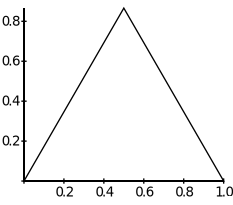
\includegraphics{8_a_triangle}}  \end{minipage}
%\begin{minipage}{2.0in}\resizebox{!}{1.5in}{\includegraphics{Striangle_9}} \end{minipage} \hspace{0.3in} \vspace{-0.1in} \begin{minipage}{2.0in} \resizebox{!}{1.6in}{\includegraphics{triangle}}  \end{minipage}
\caption{Left: An approximation of the Sierpinski triangle. Right: A triangle.}
\label{F:Striangle}
\end{center}
\end{figure}
To make this figure, we need to identify linear transformations that can be put together to produce the Sierpinski triangle.

\begin{pactivity} \label{act:IFS_1} Let $\vv_1 = [0 \ 0]^{\tr}$, $\vv_2 = [1 \ 0]^{\tr}$, and $\vv_3 =  \left[ \frac{1}{2} \ \frac{\sqrt{3}}{4}\right]^{\tr}$ be three vectors in the plane whose endpoints form the vertices of a triangle $P_0$ as shown at right in Figure \ref{F:Striangle}. Let $T : \R^2 \to \R^2$ be the linear transformation defined by $T(\vx) = A \vx$, where $A =  \frac{1}{2} I_2 = \frac{1}{2} \left[ \begin{array}{cc} 1&0 \\ 0&1 \end{array} \right]$. 

\ba
\item What are $T(\vv_1)$, $T(\vv_2)$, and $T(\vv_3)$? Draw a picture of the figure $T(P_0)$ whose vertices are the endpoint of these three vectors. How is $T(P_0)$ related to $P_0$? 
 
\item Since the transformation $T$ shrinks objects, we call $T$ (or $A$) a \emph{contraction mapping}). Notice that when we apply $T$ to $P_0$ it creates a smaller version of $P_0$. The next step is to use $T$ to make three smaller copies of $P_0$, and then translate these copies to the vertices of $P_0$. A translation can be performed by adding a vector to $T(P_0)$. Find $C_1$ so that $C_1(P_0)$ is a copy of $P_0$ half the size and translated so that $C_1(\vv_1) = \vv_1$. Then find $C_2$ so that $C_2(P_0)$ is a copy of $P_0$ half the size and translated so that $C_2(\vv_2) = \vv_2$. Finally, find $C_3$ so that $C_3(P_0)$ is a copy of $P_0$ half the size and translated so that $C_3(\vv_3) = \vv_3$. Draw pictures of each to illustrate. 

\ea

\end{pactivity}

Project Activity \ref{act:IFS_1} contains the information we need to create an iterated function system to produce the Sierpinski triangle. One more step should help us understand the general process.

\begin{pactivity} \label{act:IFS_2}  Using the results of Project Activity \ref{act:IFS_1}, define $P_{1,i}$ to be $C_i(P_0)$ for each $i$. That is, $P_{1,1} = C_1(P_0)$, $P_{1,2} = C_2(P_0)$, and $P_{1,3} = C_3(P_0)$. So $P_{1,i}$ is a triangle half the size of the original translated to the $i$th vertex of the original. Let $P_1 = \bigcup_{i=1}^3 P_{1,i}$. That is, $P_1$ is the union of the shaded triangles in Figure \ref{F:IFS_2}. 
\begin{figure}[h]
\begin{center}
\resizebox{!}{1.75in}{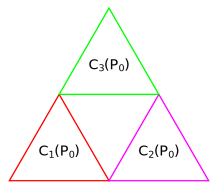
\includegraphics{8_a_IFS_2}} 
%\resizebox{!}{1.75in}{\includegraphics{IFS_2}} 
\caption{$C_1(P_0)$, $C_2(P_0)$, and $C_3(P_0)$.}
\label{F:IFS_2}
\end{center}
\end{figure}
\ba
\item Apply $C_1$ from Project Activity \ref{act:IFS_1} to $P_1$. What is the resulting figure? Draw a picture to illustrate.

\item Apply $C_2$ from Project Activity \ref{act:IFS_1} to $P_1$. What is the resulting figure? Draw a picture to illustrate.


\item Apply $C_3$ from Project Activity \ref{act:IFS_1} to $P_1$. What is the resulting figure? Draw a picture to illustrate.

\ea

\end{pactivity}

The procedures from Activities \ref{act:IFS_1} and \ref{act:IFS_2} can be continued, replacing $P_0$ with $P_1$, then $P_2$, and so on. In other words, for $i$ = 1, 2, and 3, let $P_{2,i} = C_i(P_1)$. Then let $P_2 = \bigcup_{i=1}^3 P_{2,i}$. A picture of $P_2$ is shown at left in Figure \ref{F:Striangle_2}. We can continue this procedure, each time replacing $P_{j-1}$ with $P_j$. A picture of $P_9$ is shown at right in Figure \ref{F:Striangle_2}.  
\begin{figure}[h]
\begin{center}
\resizebox{!}{1.25in}{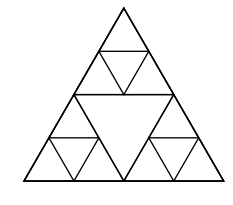
\includegraphics{8_a_Striangle_2}} \hspace{0.5in} \resizebox{!}{1.25in}{\includegraphics{8_a_Striangle_9}}
%\resizebox{!}{1.25in}{\includegraphics{Striangle_2}} \hspace{0.5in} \resizebox{!}{1.25in}{\includegraphics{Striangle_9}}
\caption{Left: $P_2$. Right: $P_9$.}
\label{F:Striangle_2}
\end{center}
\end{figure}


If we continue this process, taking the limit as $i$ approaches infinity, the resulting sequence of sets converges to a fixed set, in this case the famous Sierpinski triangle. So the picture of $P_9$ in Figure \ref{F:Striangle_2} is a close approximation of the Sierpinski triangle. This algorithm for building the Sierpinski triangle is called the \emph{deterministic algorithm}.  A Sage cell to illustrate this algorithm for producing approximations to the Sierpinski triangle can be found at \url{http://faculty.gvsu.edu/schlicks/STriangle_Sage.html}.

In general, an iterated function system (IFS)\index{iterated function system} is a finite set $\{f_1, f_2, \ldots, f_m\}$ of contraction mappings from $\R^2$ to $\R^2$. If we start with a set $S_0$, and let $S_1 = \bigcup f_i(S_0)$, $S_2 = \bigcup f_i(S_1)$, and so on, then in ``nice" cases (we won't concern ourselves with what ``nice" means here), the sequence $S_0$, $S_1$, $S_2$, $\ldots$ converges in some sense to a fixed set. That fixed set is called the  \emph{attractor}\index{attractor} of the iterated function system. It is that attractor that is the fractal. It is fascinating to note that our starting set does not matter, the same attractor is obtained no matter which set we use as $S_0$.  

One aspect of a fractal is that fractals are self-similar, that is they are made up of constituent pieces that look just like the whole. More specifically, a subset $S$ of $\R^2$ is \emph{self-similar}\index{self-similar set} if it can be expressed in the form 
\[S = S_1 \cup S_2 \cup \cdots \cup S_k\]
for non-overlapping sets $S_1$, $S_2$, $\ldots$, $S_k$, each of which is congruent to $S$ by the same scaling factor.  So, for example, the Sierpinski triangle is self-similar, made up of three copies of the whole, each contracted by a factor of $2$. 

If we have an IFS, then we can determine the attractor by drawing the sequence of sets that the IFS generates. A more interesting problem is, given a self-similar figure, whether we can construct an IFS that has that figure as its attractor. 

\begin{pactivity} \label{IFS_carpet} A picture of an emerging Sierpinski carpet is shown at left in Figure \ref{F:Scarpet}. A Sage cell to illustrate this algorithm for producing approximations to the Sierpinski carpet can be found at \url{http://faculty.gvsu.edu/schlicks/SCarpet_Sage.html}. In this activity we will see how to find an iterated function system that will generate this fractal. 
\begin{figure}[h]
\begin{center}
\resizebox{!}{2.0in}{\includegraphics{8_a_Scarpet_6}} 
%\resizebox{!}{2.0in}{\includegraphics{Scarpet_6.png}} \hspace{0.25in} \resizebox{!}{2.0in}{\includegraphics{Scarpet_6_boxes.png}}
\caption{A Sierpinski carpet.}
\label{F:Scarpet}
\end{center}
\end{figure}
\ba
\item To create an IFS to generate this fractal, we need to understand how many self-similar pieces make up this figure. Use the image at right in Figure \ref{F:Scarpet} to determine how many pieces we need. 


\item For each of the self-similar pieces identified in part (a), find a linear transformation and a translation that maps the entire figure to the self-similar piece. (Hint: You could assume that the carpet is embedded in the unit square.)


\item Test your IFS to make sure that it actually generates the Sierpinski carpet. There are many websites that allow you to do this, one of which is \url{http://cs.lmu.edu/~ray/notes/ifs/}. In this program, the mapping $f$ defined by 
\[f(\vx) = \left[ \begin{array}{cc} a&b\\c&d \end{array} \right] \vx + \left[ \begin{array}{c} e\\f \end{array}\ \right]\]
is represented as the string
\[a \ b \ c \ d \ e \ f.\]
Most programs generally use a different algorithm to create the attractor, plotting points instead of sets. In this algorithm, each contraction mapping is assigned a probability as well (the larger parts of the figure are usually given higher probabilities),  so you will enter each contraction mapping in the form
\[a \ b \ c \ d \ e \ f \ p\]
where $p$ is the probability attached to that contraction mapping. As an example, the IFS code for the Sierpinski triangle is 
\[\begin{array}{ccccccc}
0.5	&0	&0	&0.5	&0	&0		&0.33 \\
0.5	&0	&0	&0.5	&1	&0		&0.33 \\
0.5	&0	&0	&0.5	&0.5	&0.43	&0.33 
\end{array}\]

\ea

\end{pactivity}

The contraction mappings we have used so far only involve contractions and translations. But we do not have to restrict ourselves to just these types of contraction mappings. 

\begin{pactivity} \label{act:Fractal_reflection} Consider the fractal represented in Figure \ref{F:Fractal_reflection}. Find an IFS that generates this fractal. Explain your reasoning. (Hint: Two reflections are involved.) Check with a fractal generator to ensure that you have an appropriate IFS. 
\begin{figure}[h]
\begin{center}
\resizebox{!}{2.0in}{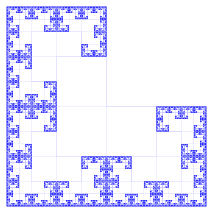
\includegraphics{8_a_Reflection_fractal}}
%\resizebox{!}{2.0in}{\includegraphics{Reflection_fractal}}
\caption{A fractal.}
\label{F:Fractal_reflection}
\end{center}
\end{figure}

\end{pactivity}

We conclude our construction of fractals with one more example. The contraction mappings in iterated function can also involve rotations. 

\begin{pactivity} \label{act:Fractal_dragon} Consider the L\'{e}vy Dragon fractal shown at left in Figure \ref{F:Fractal_rotation}. Find an IFS that generates this fractal. Explain your reasoning. (Hint: Two rotations are involved -- think of the fractal as contained in a blue triangle as shown at right in Figure \ref{F:Fractal_rotation}.) Check with a fractal generator to ensure that you have an appropriate IFS. 
\begin{figure}[h]
\begin{center}
\resizebox{!}{1.35in}{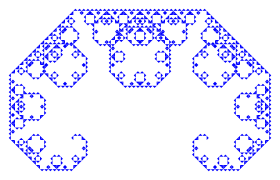
\includegraphics{8_a_Rotation_fractal}} \hspace{0.1in} \resizebox{!}{1.35in}{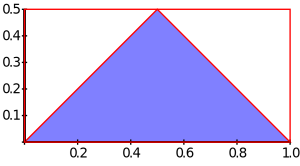
\includegraphics{8_a_Rotation_triangles}}
%\resizebox{!}{1.35in}{\includegraphics{Rotation_fractal}} \hspace{0.1in} \resizebox{!}{1.35in}{\includegraphics{Rotation_triangles}}
%crop graphics in animate trim=<left> <bottom> <right> <top>, clip with includegraphics
\caption{The L\'{e}vy Dragon.}
\label{F:Fractal_rotation}
\end{center}
\end{figure}

\end{pactivity}


We end this project with a short discussion of fractal dimension. The fractals we have seen are very strange in many ways, one of which is dimension. We have studied the dimensions of subspaces of $R^n$ -- each subspace has an integer dimension that is determined by the number of elements in a basis. Fractals also have a dimension, but the dimension of a fractal is generally not an integer. To try to understand fractal dimension, notice that a line segment is self-similar. We can break up a line segment into 2 non-overlapping line segments of the same length, or 3, or 4, or any number of non-overlapping segments of the same length. A square is slightly different. We can partition a square into 4 non-overlapping squares, or 9 non-overlapping squares, or $n^2$ non-overlapping squares for any positive integer $n$ as shown in Figure \ref{F:Squares}.
\begin{figure}[h]
\begin{center}
\resizebox{!}{1.5in}{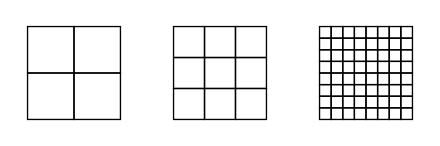
\includegraphics{8_a_similar}}
%\resizebox{!}{0.75in}{\includegraphics{square_4}} \hspace{0.5in} \resizebox{!}{0.75in}{\includegraphics{square_9}} \hspace{0.5in} \resizebox{!}{0.75in}{\includegraphics{square_64}}
\caption{Self-similar squares.}
\label{F:Squares}
\end{center}
\end{figure}
Similarly, we can break up a cube into $n^3$ non-overlapping congruent cubes. A line segment lies in a one-dimensional space, a square in a two-dimensional space, and a cube in the three-dimensional space. Notice that these dimensions correspond to the exponent of the number of self-similar pieces with scaling $n$ into which we can partition the object. We can use this idea of dimension in a way that we can apply to fractals. Let $d(\text{object})$ be the dimension of the object. We can partition a square into $n^2$ non-overlapping squares, so 
\[d(\text{square}) = 2 = 2\frac{\ln(n)}{\ln(n)} = \frac{\ln(n^2)}{\ln(n)} = \frac{\ln(\text{number of self-similar pieces})}{\ln(\text{scaling factor})}.\]
Similarly, for the cube we have 
\[d(\text{cube}) = 3 = 3\frac{\ln(n)}{\ln(n)} = \frac{\ln(n^3)}{\ln(n)} = \frac{\ln(\text{number of self-similar pieces})}{\ln(\text{scaling factor})}.\]
We can then take this as our definition of the dimension of a self-similar object, when the scaling factors are all the same (the fern fractal in Figure \ref{F:Fern} is an example of a fractal generated by an iterated function system in which the scaling factors are not all the same).

\begin{definition} The \textbf{fractal} or \textbf{Hausdorff}\index{Hausdorff dimension} dimension $h$ of a self-similar set $S$ is 
\[h(S) = \frac{\ln(\text{number of self-similar pieces})}{\ln(\text{scaling factor})}.\]
\end{definition}

\begin{pactivity} \label{act:IFS_dimension} Find the fractal dimensions of the Sierpinski triangle and the Sierpinski carpet. These are well-known and you can look them up to check your result. Then find the fractal dimension of the fractal with IFS
\[\begin{array}{ccccccc}
0.38 &0 &0 &0.38 &-0.59 	&0.81	&0.2 \\
0.38 &0 &0 &0.38 &-0.95 	&-0.31 	&0.2 \\
0.38 &0 &0 &0.38 &0 	&-1 		&0.2 \\
0.38 &0 &0 &0.38 &0.95 	&-0.31 	&0.2 \\
0.38 &0 &0 &0.38 &0.59 	&0.81 	&0.2
\end{array}.\]
You might want to draw this fractal using an online generator. 


\end{pactivity}


